\documentclass[english,handout]{beamer}






 
%\usepackage{mathptmx}
%\renewcommand{\sfdefault}{lmss}
\usepackage[T1]{fontenc}
%\usepackage[latin9]{inputenc}
\usepackage[utf8]{inputenc}

\synctex=-1

\usefonttheme{professionalfonts}

%\setbeamertemplate{navigation symbols}{}
%\setbeamertemplate{caption}[numbered]


\useinnertheme{rectangles}
%http://tex.stackexchange.com/questions/11168/change-bullet-style-formatting-in-beamer

 \AtBeginDocument{
  \addtolength\abovedisplayskip{-0.4\baselineskip}%
  \addtolength\belowdisplayskip{-0.4\baselineskip}%
}%change the space between text lines and the math formula


\usepackage{pifont}
%Postscript ZipfDingbats font
%the command \ding{number}, will print the specified symbol

\usepackage{fontawesome}
%icon package
\DeclareFontFamily{U}{FontAwesomeOne}{}
\DeclareFontShape{U}{FontAwesomeOne}{m}{n}{<-> FontAwesome--fontawesomeone}{}
\DeclareRobustCommand\FAone{\fontencoding{U}\fontfamily{FontAwesomeOne}\fontseries{m}\fontshape{n}\selectfont}
\DeclareFontFamily{U}{FontAwesomeTwo}{}
\DeclareFontShape{U}{FontAwesomeTwo}{m}{n}{<-> FontAwesome--fontawesometwo}{}
\DeclareRobustCommand\FAtwo{\fontencoding{U}\fontfamily{FontAwesomeTwo}\fontseries{m}\fontshape{n}\selectfont}
\DeclareFontFamily{U}{FontAwesomeThree}{}
\DeclareFontShape{U}{FontAwesomeThree}{m}{n}{<-> FontAwesome--fontawesomethree}{}
\DeclareRobustCommand\FAthree{\fontencoding{U}\fontfamily{FontAwesomeThree}\fontseries{m}\fontshape{n}\selectfont}

%ftp://ftp.dante.de/tex-archive/fonts/fontawesome/doc/fontawesome.pdf
%http://tug.ctan.org/info/symbols/comprehensive/symbols-a4.pdf


\usepackage{amsmath,amssymb,amsfonts,bm,mathrsfs,mathtools}

\usepackage{tikzsymbols}
%\usepackage[tikz]{bclogo}



\usepackage{perpage}
\MakePerPage{footnote} %reset for each page
%\renewcommand{\thefootnote}{\fnsymbol{footnote}} %use symbol, limit less than 9 symbols



%%%% HIGHTLIGHT  and annotation &=%%%%%%%%
\usepackage{color,xcolor}
 \usepackage{todonotes}

\usepackage[normalem]{ulem}

\usepackage[many]{tcolorbox}

\tcbset{fonttitle=\scriptsize}
\tcbset{highlight math style={enhanced,
  colframe=red!40!black,colback=yellow!20!white,arc=2pt,boxrule=.2pt,
  }}
  \newtcbox{\otherbox}[1][]{nobeforeafter,math upper,tcbox raise base,
enhanced,frame hidden,boxrule=0pt,interior style={top color=green!10!white,
bottom color=green!10!white,middle color=green!50!yellow},
fuzzy halo=1pt with green,#1}
%%\tcbhighmath{math here}
%% \otherbox{math here}



%%%%% HIGHLIGHT %%%%%%
\newcommand{\hb}[1]{{\color{blue}{#1}}}
%\noindent\rule{\textwidth}{.5pt}

%:
\usepackage{soul}

\newcommand\hcancel[2][black]{\setbox0=\hbox{$#2$}%
\rlap{\raisebox{.45\ht0}{\textcolor{#1}{\rule{\wd0}{1pt}}}}#2}
%cross to delete

\newcommand{\mcb}[2]{\colorbox{#1}{$\displaystyle #2$}}
%highlight math

\newcommand{\hlfancy}[2]{\sethlcolor{#1}\hl{#2}}
%specified color , for\hl

\newcommand\myhl{\bgroup\markoverwith
  {\textcolor{yellow}{\rule[-.5ex]{2pt}{2.5ex}}}\ULon}



\mode<presentation>{ \usetheme{boxes} }

%write Matlab code
\usepackage{listings}
 \definecolor{dkgreen}{rgb}{0,0.6,0}
\definecolor{gray}{rgb}{0.5,0.5,0.5}
\definecolor{mauve}{rgb}{0.58,0,0.82}
\lstset{frame=tb,
  language=Matlab,
  aboveskip=3mm,
  belowskip=3mm,
  showstringspaces=false,
  columns=flexible,
  basicstyle={\small\ttfamily},
  numbers=none,
  numberstyle=\tiny\color{gray},
  keywordstyle=\color{blue},
  commentstyle=\color{dkgreen},
  stringstyle=\color{mauve},
  breaklines=true,
  breakatwhitespace=true
  tabsize=3
}

\usepackage[lastexercise]{exercise}

\newtheorem{ex}{Exercise}
\newtheorem{property}{Property}
\newtheorem{ag}{Algorithm}
\newtheorem{remark}{Remark}
\newtheorem{den}{definition}
\newtheorem{assumption}{Assumption}


\usepackage[nosolutionfiles]{answers}
\Newassociation{sol}{Solution}{ans}



\usepackage{empheq}
\usepackage{comment}
%\usepackage{lscape}
\usepackage{multirow}
\usepackage{url,hyperref}

\hypersetup{
 %   bookmarks=true,         % show bookmarks bar?
    unicode=false,          % non-Latin characters in Acrobat's bookmarks
    pdftoolbar=true,        % show Acrobat's toolbar?
    pdfmenubar=true,        % show Acrobat's menu?
    pdffitwindow=false,     % window fit to page when opened
    pdfstartview={FitH},    % fits the width of the page to the window
    pdftitle={My title},    % title
    pdfauthor={Author},     % author
    pdfsubject={Subject},   % subject of the document
    pdfcreator={Creator},   % creator of the document
    pdfproducer={Producer}, % producer of the document
    pdfkeywords={keyword1} {key2} {key3}, % list of keywords
    pdfnewwindow=true,      % links in new window
    colorlinks=true,       % false: boxed links; true: colored links
    linkcolor=red,          % color of internal links (change box color with linkbordercolor)
    citecolor=green,        % color of links to bibliography
    filecolor=magenta,      % color of file links
    urlcolor=cyan           % color of external links
}


\usepackage{subfigure,epsfig,graphicx,graphics}

\DeclareGraphicsRule{.tif}{png}{.png}{`convert #1 `dirname #1`/`basename #1 .tif`.png}
   \DeclareGraphicsExtensions{.pdf}




\newcommand{\hw}{ {\underline{\tt Homework }} }
\newcommand{\hws}{ {\underline{\tt Homework$\star$}} }
\newcommand{\optional}{ {\it optional} }

\newcommand{\MATLAB}{ \texttt{MATLAB}}
\newcommand{\python}{ \texttt{python}}
\newcommand{\Rlang}{ \texttt{R}}
\newcommand{\SAS}{ \texttt{SAS}}
\newcommand{\MC}{Markov Chain}


\newcommand{\tm}{transition matrix}
\newcommand{\rv}{random variable}
\newcommand{\spl} {supervised learning }
 

\newcommand{\dis}{\underline{\tt discussion}: }
\newcommand{\pri}{\underline{\tt principle}: }




\newcommand{\bq}{\scalebox{6}{\textbf{?} }}
\newcommand{\sq}{\scalebox{2}{\textbf{?} }}
\newcommand{\ck} {  {\scalebox{0.8} {\Interval}   } }

\newcommand{\eps}{\varepsilon}
\newcommand{\To}{\longrightarrow}

% 
\newcommand{\Dcal}{\mathtt{D}}
\newcommand{\Hcal}{\mathcal{H}}
\newcommand{\Ecal}{\mathcal{E}}
\newcommand{\Xcal}{\mathcal{X}}
\newcommand{\Ycal}{\mathcal{Y}}
\newcommand{\Zcal}{\mathcal{Z}}

%%Calculus 

\renewcommand{\d}{\ensuremath{\mathrm{d}}}
\newcommand{\dt}{ \ensuremath{\mathrm{d} t } }
\newcommand{\dx}{ \ensuremath{\mathrm{d} x} }
\newcommand{\dy}{ \ensuremath{\mathrm{d} y } }

%indicator function
\newcommand{\indf}{ \ensuremath{\mathbf{1} } }



%probability
\newcommand{\p}{ \mathbb{P}}
\newcommand{\prob}{{\Pr}}
\newcommand{\PP}{\mbox{PP}}%Poisson process
%condition prob
\newcommand{\cPr}[2]{{\Pr\left(#1\mid #2\right)}}

\newcommand{\FF}{{\mathbb{F}}}

\newcommand{\e}{ \operatorname{\mathbb E}}
\newcommand{\Var}{\operatorname{\mathbb{V} }}
\newcommand{\var}{\operatorname{\text{Var} }}
\newcommand{\MSE}{\operatorname{\text{MSE} }}

\newcommand{\Std}{\operatorname{std}}
\newcommand{\Cov}{\operatorname{cov}}

%Matrix  %mathbf
\newcommand{\Pb}{{\mathbf{P}}}
\newcommand{\Qb}{{\mathbf{Q}}}
\newcommand{\Mb}{{\mathbf{M}}}
\newcommand{\cb}{\mathbf{c}}
\newcommand{\bb}{{\mathbf{b}}}

\newcommand{\Tb}{\mathbf{T}}

\newcommand{\Wb}{\mathbf{W}}
\newcommand{\wb}{\mathbf{w}}
\newcommand{\Xb}{\mathbf{X}}

\newcommand{\xb}{\mathbf{x}}

\newcommand{\Wtn}{\mathbb{W}}
\newcommand{\btn}{\mathbf{b}}



\newcommand{\eye}{{\mathbf{I}}}
%identity matrix
\newcommand{\onem}{{\mathbb{1}}}
\newcommand{\idor}{\mathbf{1}}
\newcommand{\ii}{\mathbf{i}}
%imaginary symbol

\usepackage{tikz}

%State number
\newcommand{\snum}[1]{ \raisebox{.5pt}{\textcircled{\raisebox{-.9pt} {#1}}}}

 \usetikzlibrary{arrows}
\usetikzlibrary{shapes}

%\newcommand{\snum}[1]{%
 % \tikz[baseline=(char.base)]\node[anchor=south west, draw,rectangle, rounded corners, inner sep=1.4pt, minimum size=5mm,
   % text height=1.3mm](char){\ensuremath{#1}} ;}

\newcommand*\circled[1]{\tikz[baseline=(char.base)]{
            \node[shape=circle,draw,inner sep=.4pt] (char) {#1};}}


%real number
\newcommand{\Real}{{\mathbb{R}}}
%integer
\newcommand{\ZZ}{\mathbb{Z}}
%positive integer
\newcommand{\NN}{\mathbb{N}}



\newcommand{\inpd}[2]{\left\langle #1, #2 \right\rangle}
\newcommand{\abs}[1]{\left\vert#1\right\vert}
\newcommand{\norm}[1]{\left\|#1\right\|}
\newcommand{\wt}[1]{{\widetilde{#1}}}
\newcommand{\set}[1]{\left\{#1\right\}}
\newcommand{\partiald}[2]{  \frac{\partial #1 }{\partial #2}}



\newcommand{\ie}{{\it{i.e.}}}



\newcommand{\transpose}{\textsf{T}} % or, \intercal
\newcommand{\diag}{\textsf{diag}}
\newcommand{\tr}{{\textsf{T}}}
\newcommand{\rt}{{\textbf{r}}}

\DeclareMathOperator{\trace}{Trace}


\newcommand{\argmin}{ \operatornamewithlimits{argmin} }
\newcommand{\argmax}{ \operatornamewithlimits{argmax} }




\def\biz{\begin{itemize} }
\def\bizp{\begin{itemize}[<+->] }
\def\eiz{\end{itemize}}


\def\bfm{\begin{frame}}
\def\efm{\end{frame}}

\def\bena{\begin{enumerate}[<+-| alert@+>]}
\def\ben{\begin{enumerate}}
\def\een{\end{enumerate}}


\def\bbk{\begin{block} }
\def\ebk{\end{block}}






\makeatletter
%%%%%%%%%%%%%%%%%%%%%%%%%%%%%% Textclass specific LaTeX commands.
 % this default might be overridden by plain title style

%%%%%%%%%%%%%%%%%%%%%%%%%%%%%% User specified LaTeX commands.
%\usetheme{Warsaw}
\usetheme{Boadilla}
% or ...



%\setbeamertemplate{footline}[text line]{} % makes the footer EMPTY
%\setbeamertemplate{footline}[page number]{} % makes the footer EMPTY

%\usecolortheme{orchid} %not use is better 

\setbeamertemplate{footline}[text line]{%
  \parbox{\linewidth}{\vspace*{-2pt}Xiang Zhou\hfill CityU\hfill \insertpagenumber}}
%\setbeamertemplate{navigation symbols}{}

%\setbeamercovered{transparent}
% or whatever (possibly just delete it)


%\usepackage{babel}
\makeatother



 %
%\addtobeamertemplate{frametitle}{}{%
%\begin{tikzpicture}[remember picture,overlay]
%\node[anchor=south east,yshift=2pt] at (current page.south east) {
\includegraphics[height=0.6cm]{CityU_Logo_Basic_Signature.eps}};
%\end{tikzpicture}}
%

\beamerdefaultoverlayspecification{<+->}
%the presentation acts as though a \pause command has been inserted between every two bullets, without the actual need to write \pause after each item.




\newcommand{\XX}{{X^\tr X}}
\newcommand{\bh}{{\hat{\beta} }}
\DeclareMathOperator{\Proj}{Proj}

\theoremstyle{definition}

\newtheorem*{defn}{Definition}
\newtheorem*{thm}{Theorem}
\newtheorem*{lem}{Lemma}


\title{Linear  Regression: 
Ordinary Least Square}

\author{Xiang Zhou  \\ $\ $ \\
}
\institute[]{  School of Data Science 
\\
 Department of Mathematics
\\
City University of Hong Kong
\\
~~
\\

\includegraphics[height=1.1cm,width=2.2cm]{../CityU_Logo_Basic_Signature.eps}
\\ $\ $ \\

\textup{  }
}

\date[]{}



\begin{document}
 \maketitle

 
\frame{


{\color{blue} \huge 
  Ordinary  Linear Regression}

}

 \frame{
 {Review of linear regression (univariate and multivariate )}

\biz
\item Least-square:  is usually \href{https://projecteuclid.org/download/pdf_1/euclid.aos/1176345451}{credited to Carl Friedrich Gauss} (1795), but it was first published by Adrien-Marie Legendre (1805).  \href{https://www.jstor.org/stable/pdf/2635472.pdf}{history note}.
The approach was first successfully applied to problems in 
{\bf astronomy}.

\item Loss function: squared error loss $\ell (y, \hat {y})=\abs{y-\hat{y}}^2$
\item Hypothesis  space (model class): linear function (affine function with
intercept)
\eiz
}

\frame{
{  History note : ``method of least squares'' by Gauss and Legendre}
Based on   d'Alembert’s principle, Gauss derived 
{\it Principle of least constraint}: 
\[
Z =\sum_{i=1}^N  \frac{1}{2m_i} (\bm F_i-m_i \bm A_i)^2
\]
$\bm F_i$ and $\bm A_i$ are the forces and accelerations, respectively. 
For free particles, it recovers the classic Newton's motion $\bm F_i = m_i \bm A_i$.
If constraints prevent the free choice of the $\bm A_i$, we can still minimize  $Z$ under the given auxiliary conditions. The solution obtained yields the actual motion of the system realized in nature.
\begin{example}
A particle is  forced to stay on the surface   $z=c(x,y)$ by the action of the force $\bm F$. 
Find the motion of the equation.
Hint:    $\dot{z}=c_x \dot{x}+c_y \dot{y}$ and 
$\ddot{z}=c_x \ddot{x} + c_{xx}\dot{x}^2 + c_{yy} \ddot{y} + c_{yy}\dot{x}^2
\approx c_x\ddot{x} + c_y \ddot{y} $.
The constraint for $\bm A=(\ddot{x},\ddot{y},\ddot{z})$ is
the linear equation $\ddot{z}=c_x\ddot{x} + c_y \ddot{y} $.

\end{example}

  }
 
 
 
 
 
%%%--------------------------------------------------------------------

\frame {

\frametitle{Simple linear regression}

Data $(x_1, y_1),\ldots, (x_n, y_n)$, where
\begin{itemize}
\item $x_i$ is the predictor (independent variable, input, feature)
\item $y_i$ is the response (dependent variable, output, outcome)
\end{itemize}

\vspace{3mm}
We denote the {\it regression function} as
$$
f(x) = \e (Y|X=x).
$$

\vspace{3mm}
The linear regression model assumes a specific linear form for $f$,
$$
f(x) = \beta_0 + \beta x,
$$
which is usually thought of as an approximation to the truth.

\begin{center}
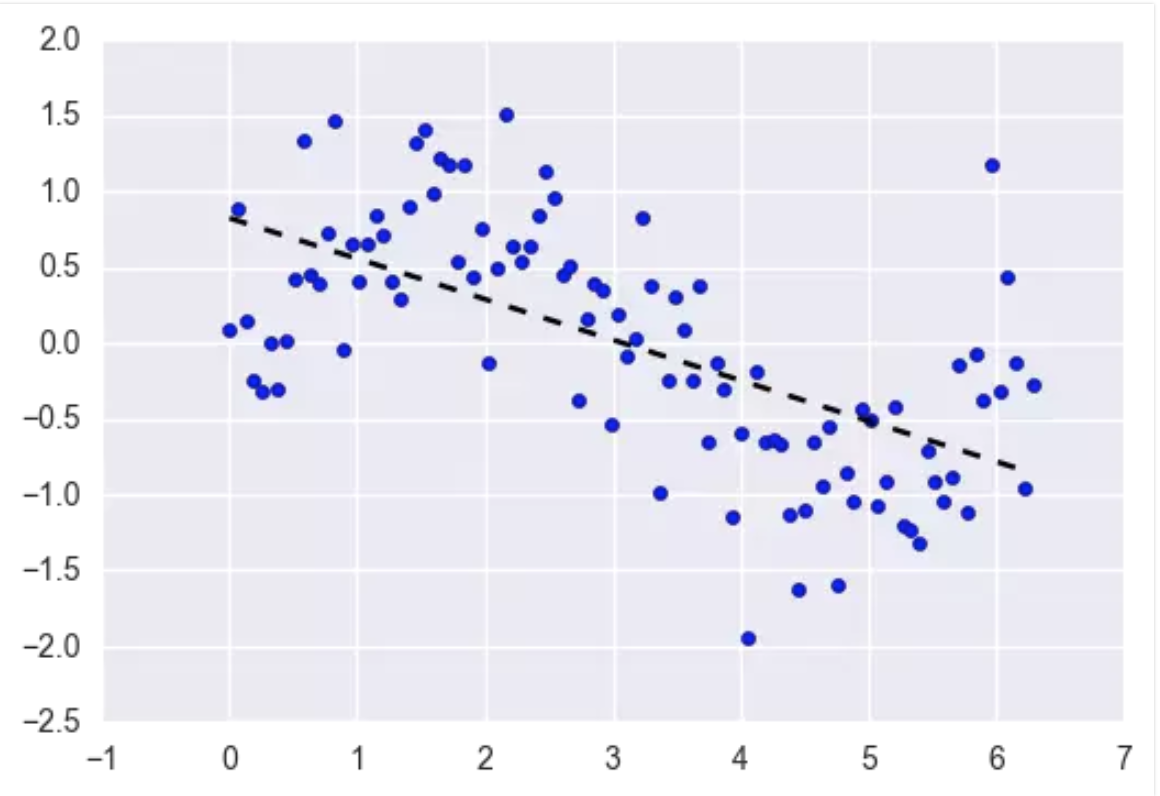
\includegraphics[width=0.45\textwidth]{pic_LR.png}
\end{center}
}



%%%--------------------------------------------------------------------

\frame {

\frametitle{Least squared fitting}

Minimize:
$$
(\hat \beta_0, \hat \beta) = \argmin_{\beta_0,\beta}~\sum_{i=1}^n (y_i-\beta_0-\beta x_i)^2.
$$

Solution is:
\begin{eqnarray*}
\hat \beta &=& \frac{\sum_{i=1}^n (x_i-\bar x)(y_i - \bar y)}{\sum_{i=1}^n (x_i-\bar x)^2}, \\
\hat \beta_0 &=& \bar y - \bar x \hat \beta.
\end{eqnarray*}

\begin{itemize}
\item $\hat y_i = \hat \beta_0 + \hat \beta x_i$ are the fitted values
\item $r_i = y_i - \hat y_i$ are the residuals
\end{itemize}

}



%%%--------------------------------------------------------------------

\frame {

\frametitle{Standard errors and confidence intervals}

Assume further that
$$
y_i = \beta_0 + \beta x_i + \epsilon_i,
$$
where $E(\epsilon_i)=0$ and $\var(\epsilon_i)=\sigma^2$. Then
$$
se(\hat \beta) = \left ( \frac{\sigma^2}{\sum (x_i - \bar x)^2} \right )^{1/2},
$$
where $\sigma^2$ can be estimated by $\hat \sigma^2 = \sum (y_i - \hat y)^2 / (n-2)$.

\vspace{3mm}
Under additional normality assumption of $\epsilon_i$'s, a $(1-\alpha)100\%$ confidence interval of $\beta$ is
$$
\hat \beta \pm z_{\alpha/2} \widehat{se}(\hat \beta).
$$
}



 
\begin{frame}{Ordinary Least Square (OLS)}


  \begin{itemize}

\item 
 The predictor variable 
$x=(x_0\equiv 1, x_1,\ldots,x_p)$ and 
{\bf Design Matrix}
\[
X=\begin{bmatrix}
 1 & x_{11} & x_{12} & \ldots  &x_{1p}  \\
 1 & x_{21} & x_{22} & \ldots &x_{2p}  \\
 &&\cdots& &\\
 1 & x_{n1} & x_{n2} & \ldots &x_{np}  \\
\end{bmatrix}\in \Real^{n\times (p+1)}.
\]
$n$ is the number of samples.
The first column $x_{i0}\equiv 1$.
\item Response vector :
$Y =\begin{bmatrix}  y_1, y_2, \ldots,y_n\end{bmatrix}^\tr$.
\par 
 
\item   Linear model  $\mathcal{H} = \set{f: f(x) = \beta^\intercal x, \beta
=(\beta_0,\beta_1,\ldots, \beta_p)\in \Real^{p+1} }$.

    \item Risk minimization view:
      \[
        \hat{\beta} = \argmin_\beta \|Y - {  X} \beta\|_2^2
        = {({  X}^\tr {  X})}^{-1} {  X}^\tr Y.
      \]

    \item Model-based interpretation:      \[
        Y =  X\beta + \varepsilon, \quad
        \varepsilon \sim \mathcal{N}(0, \sigma^2 ).
      \]
         \end{itemize}
\end{frame}

\frame{{Standarlization of Data}
The standarlization processing is helpful in many cases:
\ben
\item
Centering
\biz
\item $x_{ij} \to x_{ij}-\bar{x}_{\cdot j} $,   where $\bar{x}_{\cdot j}=\frac{1}{n}\sum_{i} x_{ij}$
\item $y_i \to y_i - \bar{y}$
\eiz
Then $\sum_{i} x_{ij}=\sum_{i} y_i =0$.
Then the intercept in OLS $\beta_0$ vanishes.
For centered data: 
$\frac{1}{n }X^\tr X = \frac{1}\sum_{i}(x_{ij} x_{ik})$ is the covariate matrix of 
the predictor.
\item
Standardization (after centering):
$$x_{ij} \to \frac{x_{ij}}{ \sqrt{\frac{1}{n} \sum_i  x_{ij}^2} }.$$
Then $\frac{1}{n}\sum_i x_{ij}^2 \equiv 1, ~\forall j$.
%It follows that $\trace(X^\tr X) = \sum_{ij} (x_{ij}^2)=n^2$
\een

}

%%%------------------------------------------------
\frame{
\ben

   \item Understanding OLS from the perspective of  
    MLE and Bayes
    
\item Understanding OLS from the perspective of 
  linear algebra:  orthogonal project,  pseudo-inverse,
  Gram-Schmidt procedure; QR, SVD
         \item Understanding uncertainty in $\hat{\beta}$ :
    variance analysis
       
    \item Understanding OSL
  as   the minimum variance unbiased estimator 
of the response : Gauss-Markov theorem


  \een
}


\begin{frame}
  {Maximum log-\emph{likelihood function}}
  \par
  $\eps\sim \mathcal{N}(0,\sigma^2)$ leads to the 
  log-likelihood function
  \begin{align*}
    \log \mathcal{L}(\beta; x_i, y_i)
    & = \log \prod_{i=1}^n p(y_i | x_i) p(x_i)
    = \sum_{i=1}^n \log p(y_i | x_i) + \sum_{i=1}^n \log p(x_i) \\
    & = \sum_{i=1}^n \log\left[
      \frac{1}{\sqrt{2 \pi \sigma^2}}
      e^{-\frac{{(y_i - \beta^\intercal x_i)}^2}{2 \sigma^2}} \right]
    + \sum_{i=1}^n \log p(x_i) \\
    & = -\frac{1}{2 \sigma^2} \sum_{i=1}^n {(y_i - \beta^\intercal x_i)}^2
    + \text{terms not depend on $\beta$}.
  \end{align*}
  Therefore $\hat{\beta}^\text{MLE} = \hat{\beta}^\text{OLS}$.

\end{frame}
 
 

\frame{
\biz
 
    
\item Understanding OLS from the perspective of 
  linear algebra:  orthogonal project,  pseudo-inverse,
  Gram-Schmidt procedure; QR, SVD
  
  \eiz
}


 \frame{
 {OLS prediction as the  orthogonal projection}
 \biz
 \item
 The optimal  prediction 
\begin{equation} \hat{Y}= X\hat{\beta}=X(X^\tr X)^{-1} X^\tr Y
=: \tcbhighmath{\Proj_{\mathsf{X}} Y}
\end{equation}
 is the orthogonal projection of the vector $Y\in \Real^n$ onto the subspace
 spanned by 
the $p+1$ column vectors of the matrix $X$
$$\mathsf{X}=\mbox{span}\{X_0, X_1, \ldots, X_p \}$$

\item
 $\hat{Y}$ is the point in $\Real^n$ with the shortest Euclidian distance 
to this subspace $\mathsf{X}$.

\item
It would be nice if we have a set of $p+1$ {\em orthonormal basis vector} of   $\mathsf{X}$.
This can be done  by Gram-Schmidt procedure (Sec. 3.2.3. in [ESL]
under the name ``sequential linear regression'') .
\item
In addition, one can use QR,  SVD decomposition of $X^\tr X$.
To efficiently find the orthogonal projection of the vector $Y$
onto a subspace spanned by $X_i$ in $\Real^n$ is a classic topic in numerical linear algebra.
 \eiz
 }

\frame{
{Properties of Projection matrix}
\[
P=\Proj_{\mathsf{X}} = X(X^\tr X)^{-1} X^\tr
\]
satisfies
\biz
\item  symmetric: $P=P^\tr$;
\item  idempotent: $P^2=\eye_n$ identity matrix;
\item  rank = $\dim(\mathsf{X})=p+1$
\item  eigenvalues:  $p+1$ ones and $n-(p+1)$ zeros;
\item  trace = $\dim(\mathsf{X})$.
\eiz

Other names used in statistics literature for the projection matrix $\Proj_{\mathsf{X}}$
\biz
\item influence matrix;
\item hat matrix
\eiz
}
%-------



\begin{frame}
{Singular Value Decomposition}
\biz
\item Assume $X= UDV^\tr$ is a SVD  of the design matrix $X$, then
 $D=\diag\set{d_0,\dots, d_{p}}$, $d_i$ is the singular value of $X$. 
 \item The column vectors of $U$, $\set{U_i, 0\leq i\leq p}$ , is a set of orthonormal basis of $\mathsf{X}$.
  \item 
Then $\XX= VD^2 V^\tr$, and  $\Proj_{\mathsf{X}} = X(\XX)^{-1}X^\tr = (UDV^\tr) VD^{-2} V^{\tr}  VDU^\tr =UU^\tr$.
\item 
\[
\hat{Y}= \Proj_{\mathsf{X}} Y=UU^\tr  Y= \sum_{i=0}^p \alpha_i U_i,
~~\mbox{ where } ~ \alpha_i  =U_i \cdot Y. 
\]

\eiz
\end{frame}

%-------

\frame{
\begin{ex}
The  projection matrix $\Proj_{\mathsf{X}}$ has the trace $p+1$.
\end{ex}
(Hint $\trace(AB)=\trace(BA)$. The eigenvalues of the projection matrix are
either 0 or 1.)

 
\begin{ex}
Exercise 3.4 in [ESL].
\end{ex}
}




\frame{
{The decomposition of sum-of-squares  }
For the OLS predicted response $ \hat{Y}= X\hat{\beta}$,  we have
 $$\otherbox{SST = SSR + SSE}$$
 \biz
 \item SST= total sum of squares for the response variable
 \[SST =  \sum_{i} (y_i - \bar{y})^2 = \norm{Y-\bar{Y}}^2_2 \]
 \item SSE=sum of squares of errors
 \footnote{[ISL] [ESL] name this as RSS= residual sum of squares}
 \[SSE =  \sum_{i} (y_i - \hat{y}_i)^2  = \| Y-\mbox{proj}_{\mathsf{X}} Y\|^2_2  \]
 \item SSR = sum of squares explained by regression
  \[SSR =  \sum_{i}(\hat{y}_i - \bar{
  \hat{y}})^2  = \norm{\hat{Y}-\bar{Y}}_2^2\]
Note that the average of the training response $\bar{y}$
is equal to the average of predicted response $\bar{\hat{y}}$
 \eiz

}


\frame{
Proof of $SST=SSE+SSR$: Exercise!
(consider $Z=Y-\bar{y}1_{n}$ and $1_{n} =X_0\in \mathsf{X}$.
consider f centered data where $\bar{y}=0$. )

\begin{ex}
Show that
\[
SSE =\norm{  (\eye_n - {\Proj}_{\mathsf{X}}) \eps }_2^2
= \norm{ {\Proj}_{\mathsf{X}^\perp}  ( \eps)  }_2^2
\]
$\eye_n - {\Proj}_{\mathsf{X}}$ is called residual marker matrix sometimes.
\end{ex}
by using $Y=X\beta +\eps$ and $\hat{Y}=\Proj_{\mathsf{X}} Y$.

Draw a picture to illustrate this result.
}
\frame{
\biz

   
    \item Understanding uncertainty in $\hat{\beta}$:
 unbiasedness,    consistence,     variance analysis
  \eiz
}



\frame{
{The distribution of the OLS coefficient $\hat{\beta}$}
Since $  Y = X\beta  + \eps$,
then\begin{align*}
 \hat{\beta}&= (X^\tr X)^{-1} X^\tr Y = (X^\tr X)^{-1} X^\tr  (X\beta  + \eps ) \\
& = \beta  + (X^\tr X)^{-1} X^\tr \eps
\end{align*}
Note that $\eps \sim N(0, \sigma^2I_{n})$, thus 
\[ \e \bh = \beta ~~~ \mbox{ (unbiased estimator)} \]
\begin{align*}
 \Var(\bh)  & = \Var( (\XX)^{-1} X^\tr  \eps)\\
&=(\XX)^{-1} X^\tr  \Var(\eps)  (\XX^{-1} X^\tr )^\tr \\
&=\sigma^2 (\XX)^{-1} X^\tr  I_n X(\XX)^{-1} \\
&=\sigma^2 (\XX)^{-1}. 
\end{align*}
Therefore, 
\[\tcbhighmath{\bh \sim
\mathcal{N}(\beta,\sigma^2 (X^\tr X)^{-1} )},\]
from which the confidence interval of $\bh$ can be calculated.
}


\frame{
{Consistency of $\bh$}
Assume that 
\[\lim _ { n \rightarrow \infty } \left( \frac { X ^ { \tr } X } { n } \right) = \Delta \]
exists as a nonstochastic and nonsingular matrix (for example,  $|x_{ji}|\leq c$ is bounded ).
Then

$$
\begin{aligned} \lim _ { n \rightarrow \infty } \e | \bh  - \beta|^2 &=
\lim _ { n \rightarrow \infty } \Var ( \bh )
\\ & = \sigma ^ { 2 } \lim _ { n \rightarrow \infty } \frac { 1 } { n } \left( \frac { X ^ { \tr } X } { n } \right) ^ { - 1 } \\ & = \sigma ^ { 2 } \lim _ { n \rightarrow \infty } \frac { 1 } { n } \Delta ^ { - 1 } \\ & = 0 \end{aligned}
$$
This implies that OLSE $\bh$ converges to in quadratic mean.
Thus OLSE $\bh$ is a consistent estimator of  $\beta$.
}
\frame{
\biz 
\item
{The distribution of $\hat{Y}=X\bh$}
is then 
$\mathcal{N}(X\beta, \sigma^2 X (\XX)^{-1}X^\tr )$
\item

When a new data of input $x$ arrives, taking value  $x_i=a_i, ~~i=1,\ldots,p$, 
with   $a=(1,a_1,a_2,\ldots,a_p)^\tr \in \Real^{p+1}$, then
 the prediction 
from the regression equation is 
\[ \hat{y} :=   a^\tr  \bh
\sim  \mathcal{N}(a^\tr \beta,~\sigma^2  a^\tr (\XX)^{-1} )a)\]
which can give the \hb{confidence interval} of  $\hat{y}=a^\tr \bh$.
\item 
But remember that in our model $Y = X\beta  + \eps$, 
 it is assumed  that the data you {\em observe}  
 inevitably is contaminated by the measurement error $\eps$.
 By including this measurement error,  the predicted 
 value at this new input $x=a$ is 
\[\hat{y} +\eps_a = a^\tr \bh +\eps_a
\]
where $\eps_a$ is  $\mathcal{N}(0,\sigma^2_a)$ and independent of the training data you used to build the regression equation.

It is clear that the distribution of  $\hat{y} +\eps_a$
is $$\mathcal{N}(a^\tr \beta,~ \sigma^2  a^\tr (\XX)^{-1} )a + \sigma^2_a),$$
which gives   the \hb{prediction interval}.


\eiz
}


\frame{ {The variance of the measurement error $\sigma^2$}
\biz
\item Recall SST is the sample variance of $Y$
then $\e SST = (n-1)\sigma^2$ 
since $\Var(Y)= \Var(\eps)=\sigma^2$.
\item 
We show below that 
$\e SSE = (n-p-1)\sigma^2$
\item 
Which one among SST and SSE should be used to define 
$\hat{\sigma}^2$, the estimate of the variance of $\eps$?

\eiz

From exercise, we have 
\[ SSE =\norm{ {\Proj}_{\mathsf{X}^\perp}  ( \eps)  }_2^2
=\eps ^\tr  ({\Proj}_{\mathsf{X}^\perp})^\tr 
(  {\Proj}_{\mathsf{X}^\perp})   \eps.
\]
where the Gaussian vector $\eps$ have variance matrix $\sigma^2 I_n$.
Since the dimension $\dim X^\perp = n - \dim (\mathsf{X}) = n-(p+1) $,
then $\trace({\Proj}_{\mathsf{X}^\perp}) = n-(p+1)$.
Then we have the conclusion 
\[
\e SSE = \trace ( ({\Proj}_{\mathsf{X}^\perp}) \sigma^2 I_{n} ) 
=(n-(p+1))\sigma^2. 
\]
}
\frame{
\begin{ex}\label{1}
Let $\mu = \e(X)$  and $\Sigma=\Var(X)$ be the mean vector and the covariance matrix of 
the random vector $X$ in $\Real^n$. $M$ is  $n\times n$ symmetric matrix. Define the random variable 
$z=(X-\mu)^\tr M(X-\mu)$, then 
\[ \e(z)=\trace(M\Sigma)=\trace(\Sigma M) \]
and thus 
\[ \e (X^\tr MX) = \trace(M\Sigma) +\mu^\tr M \mu. \]
\end{ex}
}

\frame{
\biz

   
    \item Understanding OSL
  as  the best linear unbiased estimator (BLUE) with the smallest MSE.

       \eiz
}



\frame
{  
{Gauss-Markov theorem  (Rao, 1973)
}

\biz

\item Recall the ML basics:
Given a training dataset $\Dcal$, the function to approximate
in the hypothesis space $\Hcal$  
$\hat{f}_\Dcal \in \Hcal$ is a function $x$.
In OLS, we assumed that
$\hat{f}_\Dcal=\beta^\tr x$ is a linear function of $x$ parametrized by $\beta$.
\item
Now, if we fix a testing input $x=a$ now, 
$\hat{f}_\Dcal (a)$ then is a mapping (\underline{statistics})
from $\Dcal$ to $\Ycal$.
What if we assume this mapping is linear and 
consider the  {\bf MVU}(minimum variance unbiased)  estimator of the ground truth $\beta^\tr a$ when $x=a$?
\item Fix the design matrix $X$,
then this estimator takes  the linear form
$$Y\to c^\tr Y$$ with the coefficient $c\in \Real^n$.
\eiz

}
\frame{
\begin{theorem}[Gauss-Markov Theorem]

Let $u$ be an unbiased estimate of the ground truth response $a^\tr \beta$
at the new input $x=a$ in the space of   linear transformations from the
 response  training data $Y=X\beta+\eps$,
where   $\eps\sim N(0,\sigma^2 I_n)$.
This is to say that
$u=c^\tr Y$ for some  vector $c\in \Real^{(p+1) }$
satisfies $\e u = a'\beta$  for {\em any } $\beta$ in $\Real^{p+1}$.
Then
$$\var(u) \geq \var(\hat{y}) = \sigma^2 a^\tr (\XX)^{-1}a $$ 
where $\hat{y}=a^\tr\bh^{\text{OLS}}=a^\tr (\XX)^{-1}X^\tr Y$.
 (see Exercise 3.3 in [ESL].)
\end{theorem}
\begin{proof}
$\e u = c^\tr  \e Y = c^\tr X \beta$  must equal to $a'\beta$; then
$$X'c=a.$$
$\var(u)=c^\tr \var(y)c=\sigma^2 c^\tr c $.
The optimal $c$ is the minimizer of the $L_2$ norm $\|c\|_2$
subject to the $n$ linear constraints: $X^\tr c=a$.
This is to search the $L_2$-minimal solution of the linear system $ X^\tr c =a $.
The remaining is left as an exercise.
\end{proof}
}

\frame{{Cramer-Rao low bound}
\begin{ex}
Find the Fisher information matrix, which is the 
  covariance matrix of the parameter-gradient
of the log likelihood function
$I(\beta):= \Var(\partial_\beta \log p(Y;\beta)  )$
and show that the variance matrix of $ \bh^{OLS}=(\XX)^{-1}X^\tr Y$
is the lower bound $I^{-1}(\beta)$
\end{ex}
}


\end{document}

